\clearpage
\subsubsection{Sơ đồ luồng dữ liệu DFD}
\label{aihub:sec:dfd}

Phần này trình bày sơ đồ ngữ cảnh và DFD mức 1 của AIHub, tập trung vào dữ liệu xác thực API, sinh bài, thẩm định mẫu, cấu hình và giám sát. Backend, Gateway và các kho dữ liệu thuộc phạm vi hệ thống; nhà cung cấp AI và WISPACE Reference API là các tác nhân ngoài. Nguồn dẫn chứng Writing được phân biệt với dữ liệu bài nói của Wispace Speaking.

Luồng dữ liệu được tổ chức quanh các nhóm nghiệp vụ dưới đây. Mã E, P và D chỉ có ý nghĩa trong phạm vi từng hệ thống.

\begin{longtable}{|>{\raggedright\arraybackslash}p{0.07\linewidth}|>{\raggedright\arraybackslash}p{0.25\linewidth}|p{0.58\linewidth}|}
\caption{Tác nhân ngoài của AIHub}\label{aihub:tab:dfd-entities}\\
\hline
\textbf{Mã} & \textbf{Tác nhân} & \textbf{Dữ liệu trao đổi} \\
\hline
\endfirsthead
\hline
\textbf{Mã} & \textbf{Tác nhân} & \textbf{Dữ liệu trao đổi} \\
\hline
\endhead
E1 & Người dùng Portal & Gồm lập trình viên, chuyên viên học thuật, kỹ sư AI và quản trị viên. Cung cấp thông tin đăng nhập, yêu cầu thao tác và dữ liệu cấu hình; nhận kết quả theo quyền. \\
\hline
E2 & Ứng dụng tích hợp & Gửi credentials và payload gọi API; nhận bài tập, metadata sử dụng hoặc thông tin lỗi. Không mặc định đồng nhất ứng dụng này với mô-đun Speaking. \\
\hline
E3 & Nhà cung cấp AI & Gồm WISPACE AI Micro-Engine, Gemini và OpenAI. Nhận Prompt hoặc yêu cầu thăm dò; trả nội dung sinh, metadata hoặc trạng thái. Deterministic Engine nằm trong AIHub. \\
\hline
E4 & WISPACE Reference API & Nhận bộ lọc dẫn chứng lỗi viết; trả dữ liệu ngữ cảnh IELTS Writing hoặc thông tin lỗi kết nối. \\
\hline
\end{longtable}


\begin{longtable}{|>{\raggedright\arraybackslash}p{0.07\linewidth}|p{0.48\linewidth}|p{0.35\linewidth}|}
\caption{Tiến trình mức 1 của AIHub}\label{aihub:tab:dfd-processes}\\
\hline
\textbf{Mã} & \textbf{Tiến trình} & \textbf{Phạm vi} \\
\hline
\endfirsthead
\hline
\textbf{Mã} & \textbf{Tiến trình} & \textbf{Phạm vi} \\
\hline
\endhead
P1 & Xác thực Portal và quản lý khóa & UC01--UC02 \\
\hline
P2 & Kiểm thử và xử lý API sinh bài & UC03--UC05, UC07 \\
\hline
P3 & Truy vấn dẫn chứng và thẩm định mẫu & UC06, UC08--UC11 \\
\hline
P4 & Cấu hình Prompt, model và đặc tả & UC12--UC13, UC19 \\
\hline
P5 & Phân tích chất lượng và xuất dữ liệu & UC14--UC15 \\
\hline
P6 & Quản trị tổ chức và giám sát & UC05, UC16--UC18, UC20 \\
\hline
\end{longtable}


\begin{longtable}{|>{\raggedright\arraybackslash}p{0.07\linewidth}|p{0.25\linewidth}|p{0.58\linewidth}|}
\caption{Kho dữ liệu của AIHub}\label{aihub:tab:dfd-stores}\\
\hline
\textbf{Mã} & \textbf{Kho dữ liệu} & \textbf{Nội dung} \\
\hline
\endfirsthead
\hline
\textbf{Mã} & \textbf{Kho dữ liệu} & \textbf{Nội dung} \\
\hline
\endhead
D1 & Danh tính và tổ chức & Tài khoản, phiên Portal, thành viên, vai trò, tổ chức, clientId và mã băm khóa bí mật. \\
\hline
D2 & Cấu hình dịch vụ & Prompt có phiên bản, chuỗi dự phòng, Universal Specs, gói và cấu hình hạn mức theo tổ chức. \\
\hline
D3 & Usage và kiểm toán & Sử dụng quota, mã phản hồi, latency, token và dấu vết thay đổi phục vụ giám sát, đối soát. \\
\hline
D4 & Dữ liệu học thuật & Dẫn chứng cục bộ, Prompt gắn với mẫu, rawAiOutput, finalOutput, điểm, trạng thái, người duyệt và lý do từ chối. \\
\hline
\end{longtable}


\clearpage

\paragraph{Sơ đồ ngữ cảnh.}

Sơ đồ thể hiện toàn bộ AIHub như một tiến trình duy nhất; các mũi tên ghi rõ dữ liệu gửi đến và dữ liệu trả về cho từng tác nhân ngoài.

\begin{figure}[H]
\centering
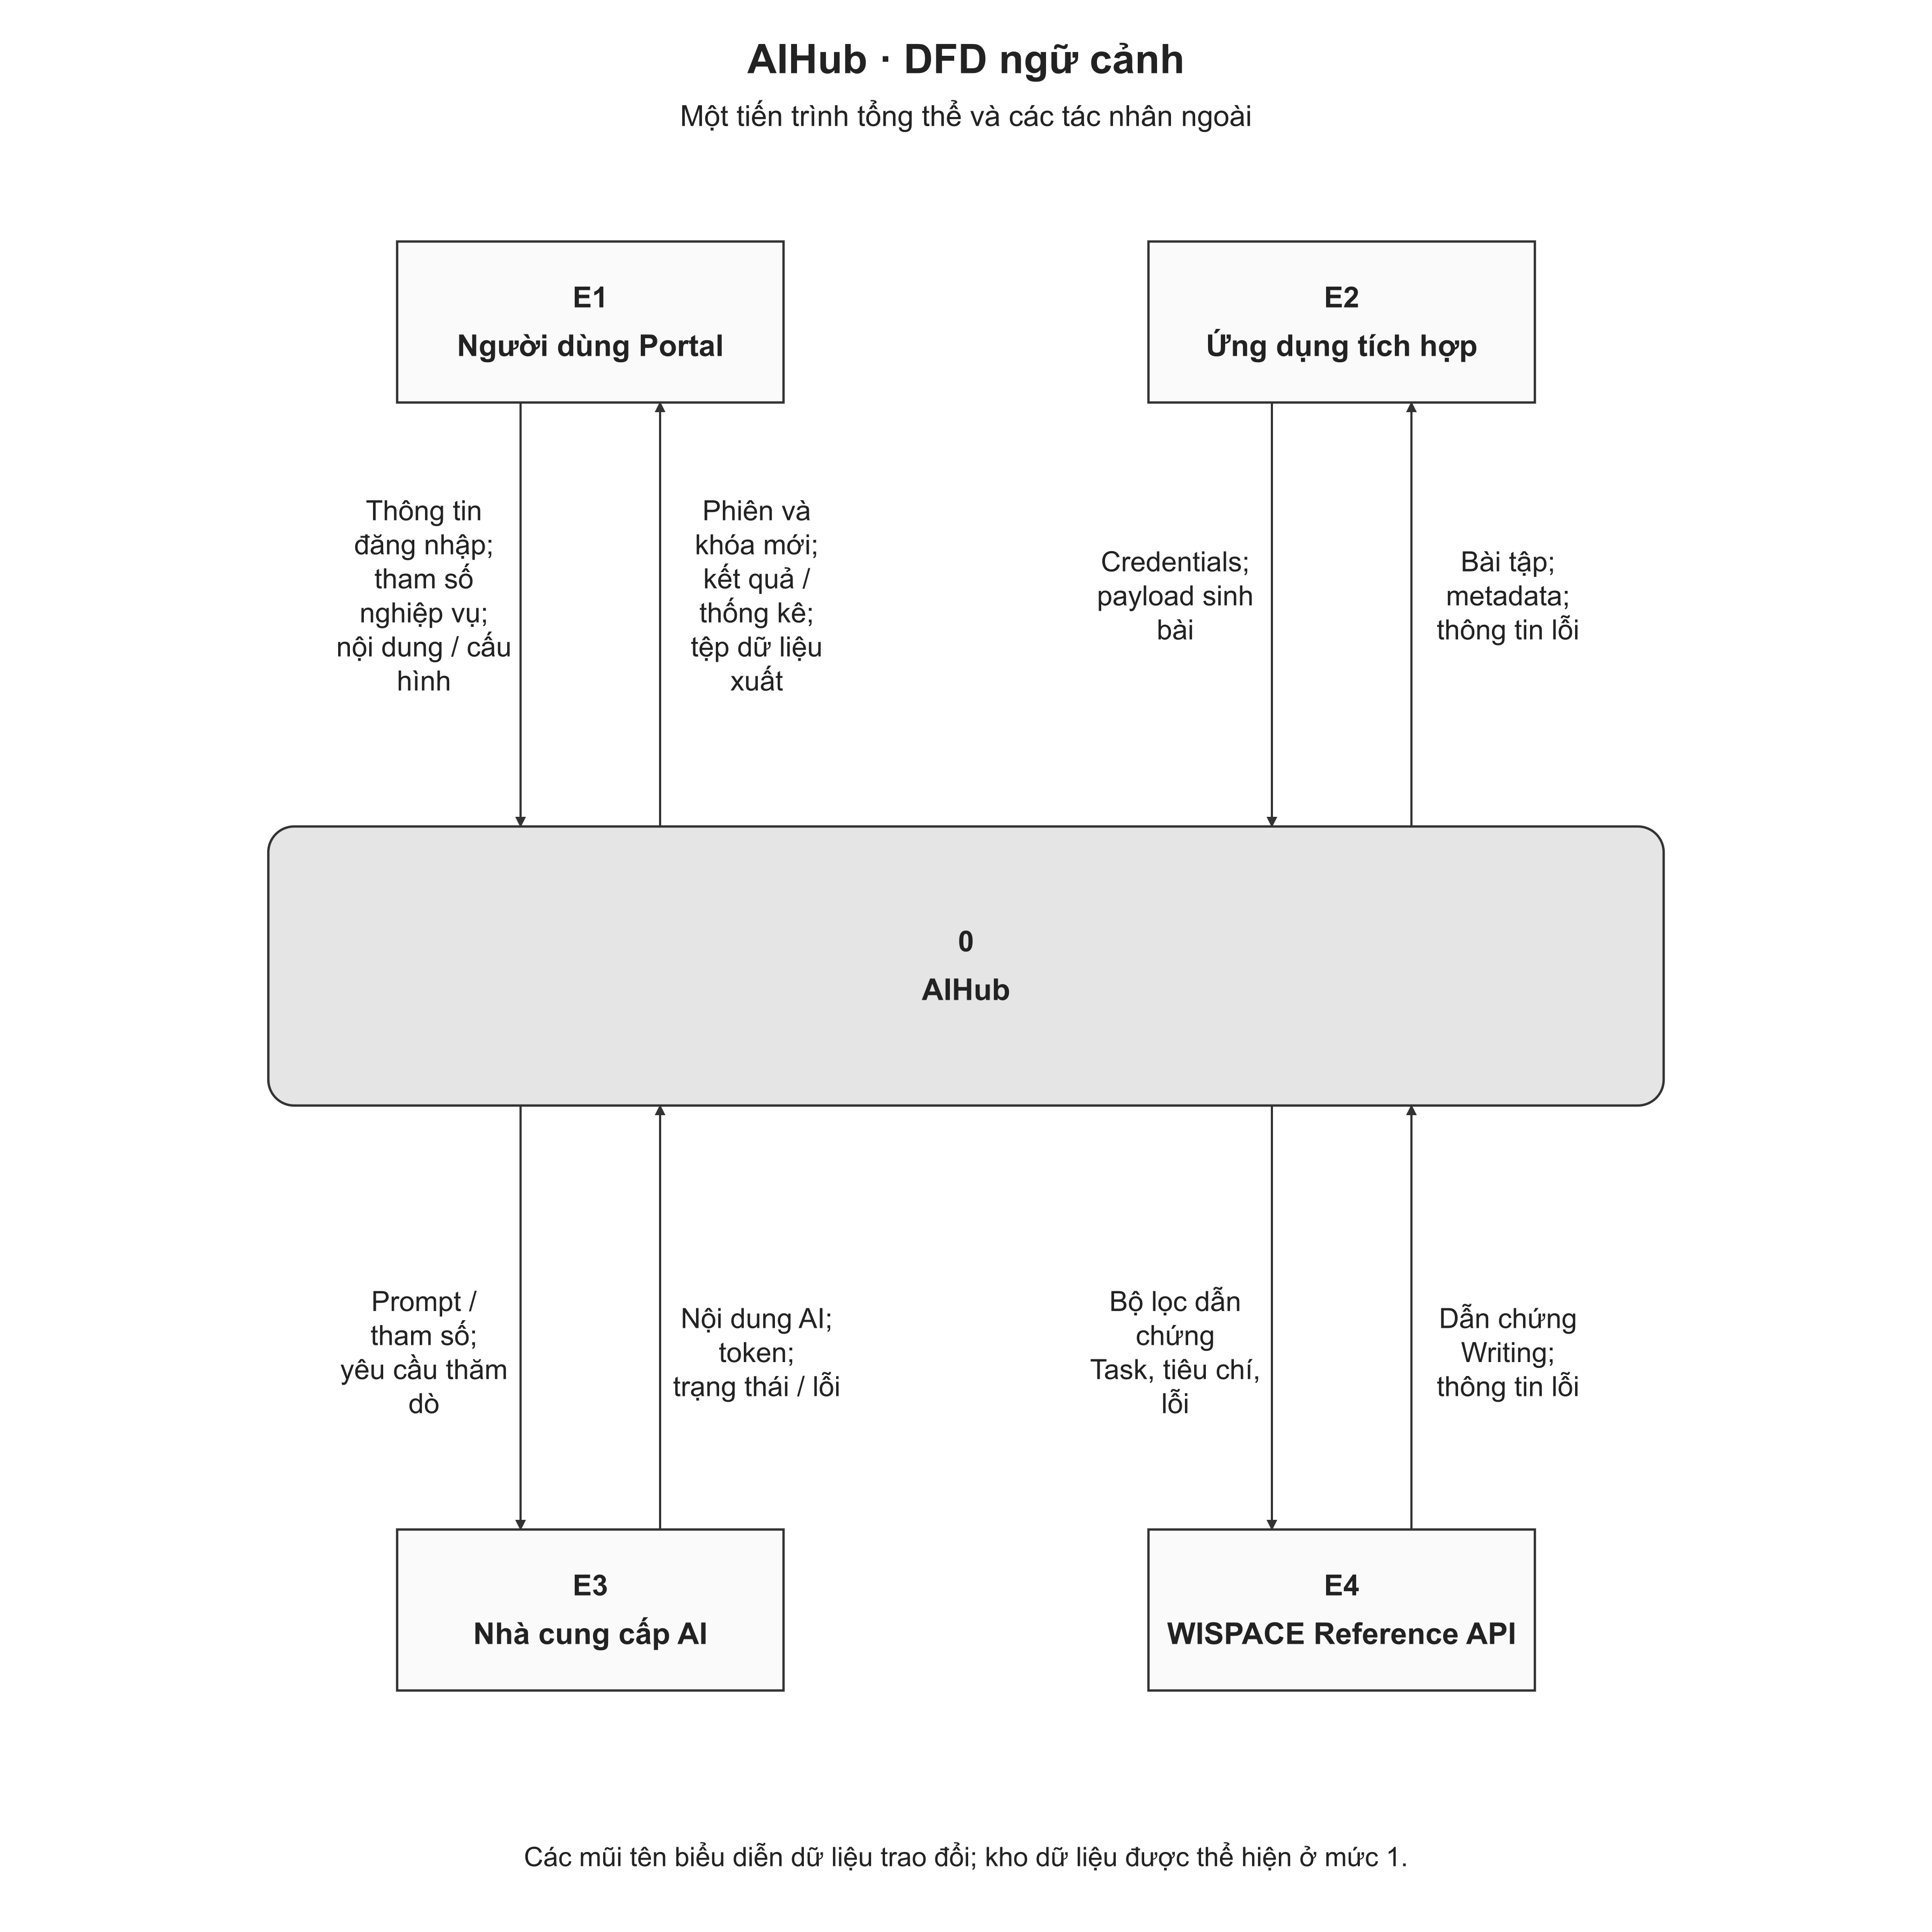
\includegraphics[width=\linewidth,height=0.78\textheight,keepaspectratio]{Images/DFD/AIHub/aihub_dfd_context.png}
\caption{DFD ngữ cảnh của AIHub}
\label{aihub:fig:dfd-context}
\end{figure}

\clearpage

\begin{longtable}{|p{0.22\linewidth}|p{0.72\linewidth}|}
\caption{Luồng dữ liệu biên của AIHub}\label{aihub:tab:dfd-boundary}\\
\hline
\textbf{Nguồn → Đích} & \textbf{Dữ liệu} \\
\hline
\endfirsthead
\hline
\textbf{Nguồn → Đích} & \textbf{Dữ liệu} \\
\hline
\endhead
E1 → 0 & Thông tin đăng nhập; tham số nghiệp vụ; nội dung / cấu hình \\
\hline
0 → E1 & Phiên và khóa mới; kết quả / thống kê; tệp dữ liệu xuất \\
\hline
E2 → 0 & Credentials; payload sinh bài \\
\hline
0 → E2 & Bài tập; metadata; thông tin lỗi \\
\hline
0 → E3 & Prompt / tham số; yêu cầu thăm dò \\
\hline
E3 → 0 & Nội dung AI; token; trạng thái / lỗi \\
\hline
0 → E4 & Bộ lọc dẫn chứng Task, tiêu chí, lỗi \\
\hline
E4 → 0 & Dẫn chứng Writing; thông tin lỗi \\
\hline
\end{longtable}


\paragraph{Sơ đồ mức 1.}

Để giữ nhãn và đường nối dễ đọc, cùng một sơ đồ mức 1 được trình bày thành hai phần. Các tác nhân và kho dữ liệu có cùng mã ở hai phần là cùng một đối tượng logic. Dữ liệu giữa các nhóm xử lý được trao đổi qua kho dùng chung, không phải các bản sao tách biệt.

\clearpage

\begin{figure}[H]
\centering
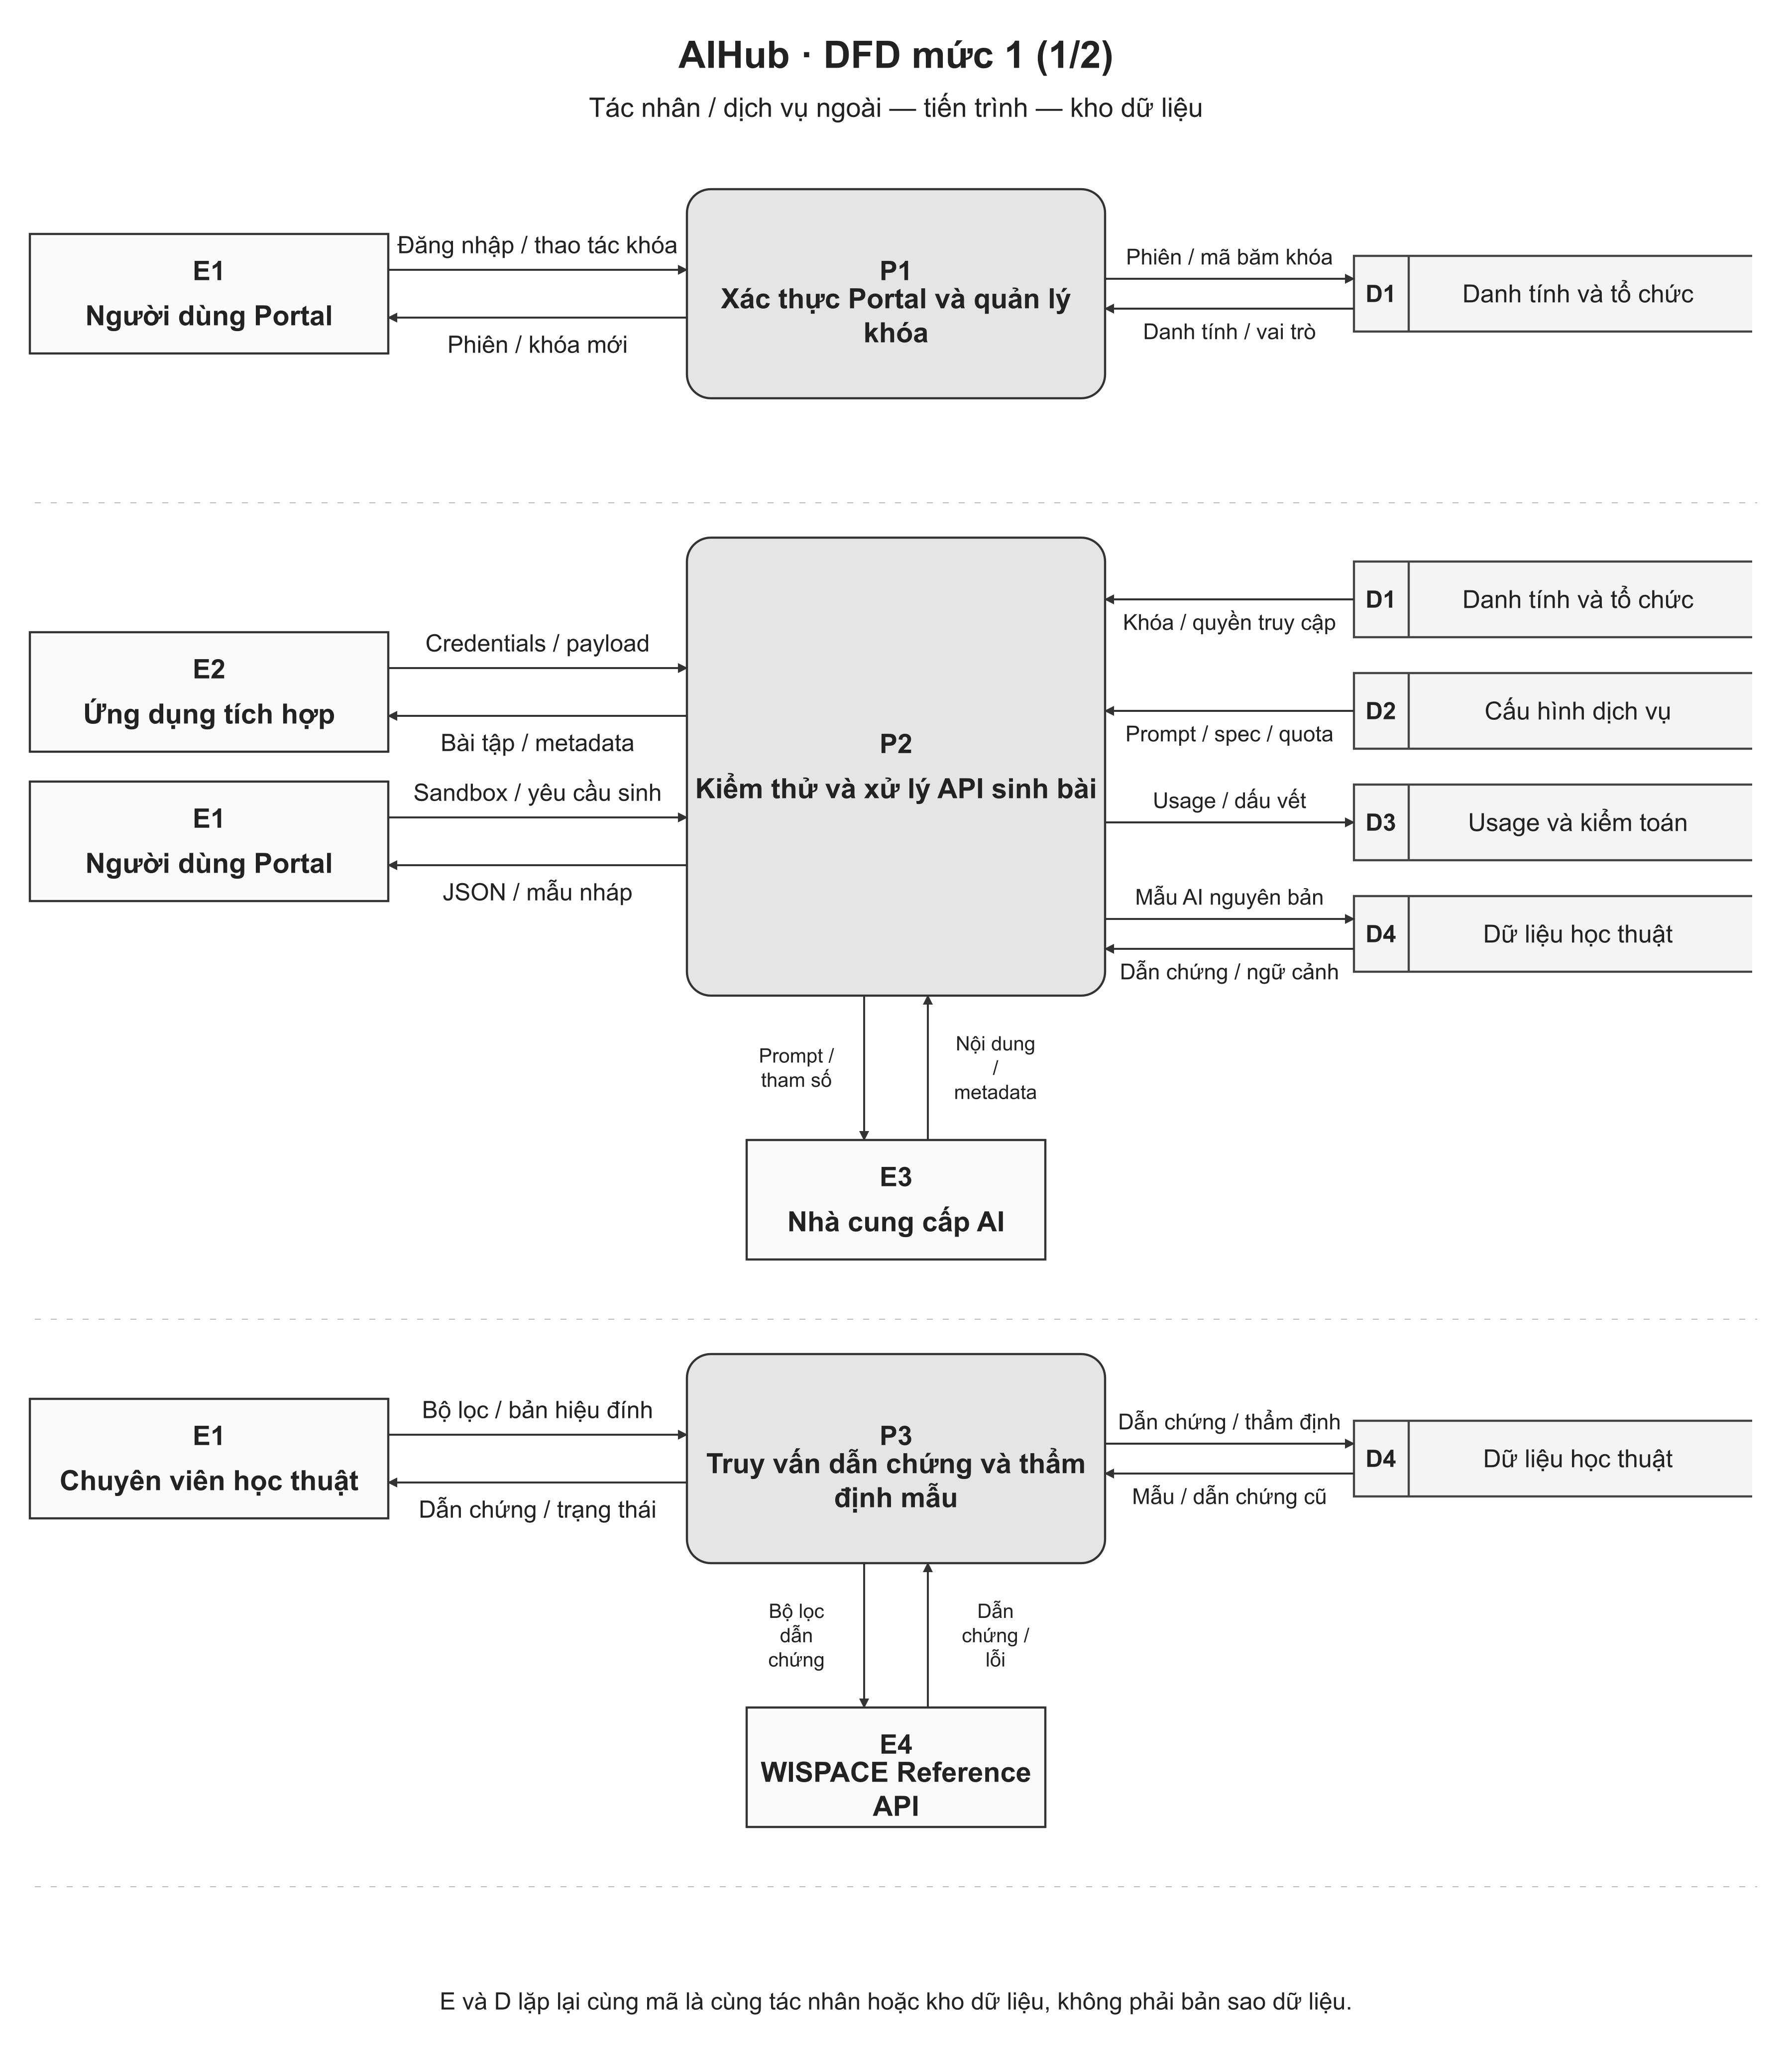
\includegraphics[width=\linewidth,height=0.78\textheight,keepaspectratio]{Images/DFD/AIHub/aihub_dfd_level1_1.png}
\caption{DFD mức 1 của AIHub: P1, P2, P3}
\label{aihub:fig:dfd-level1-1}
\end{figure}

\clearpage

\begin{figure}[H]
\centering
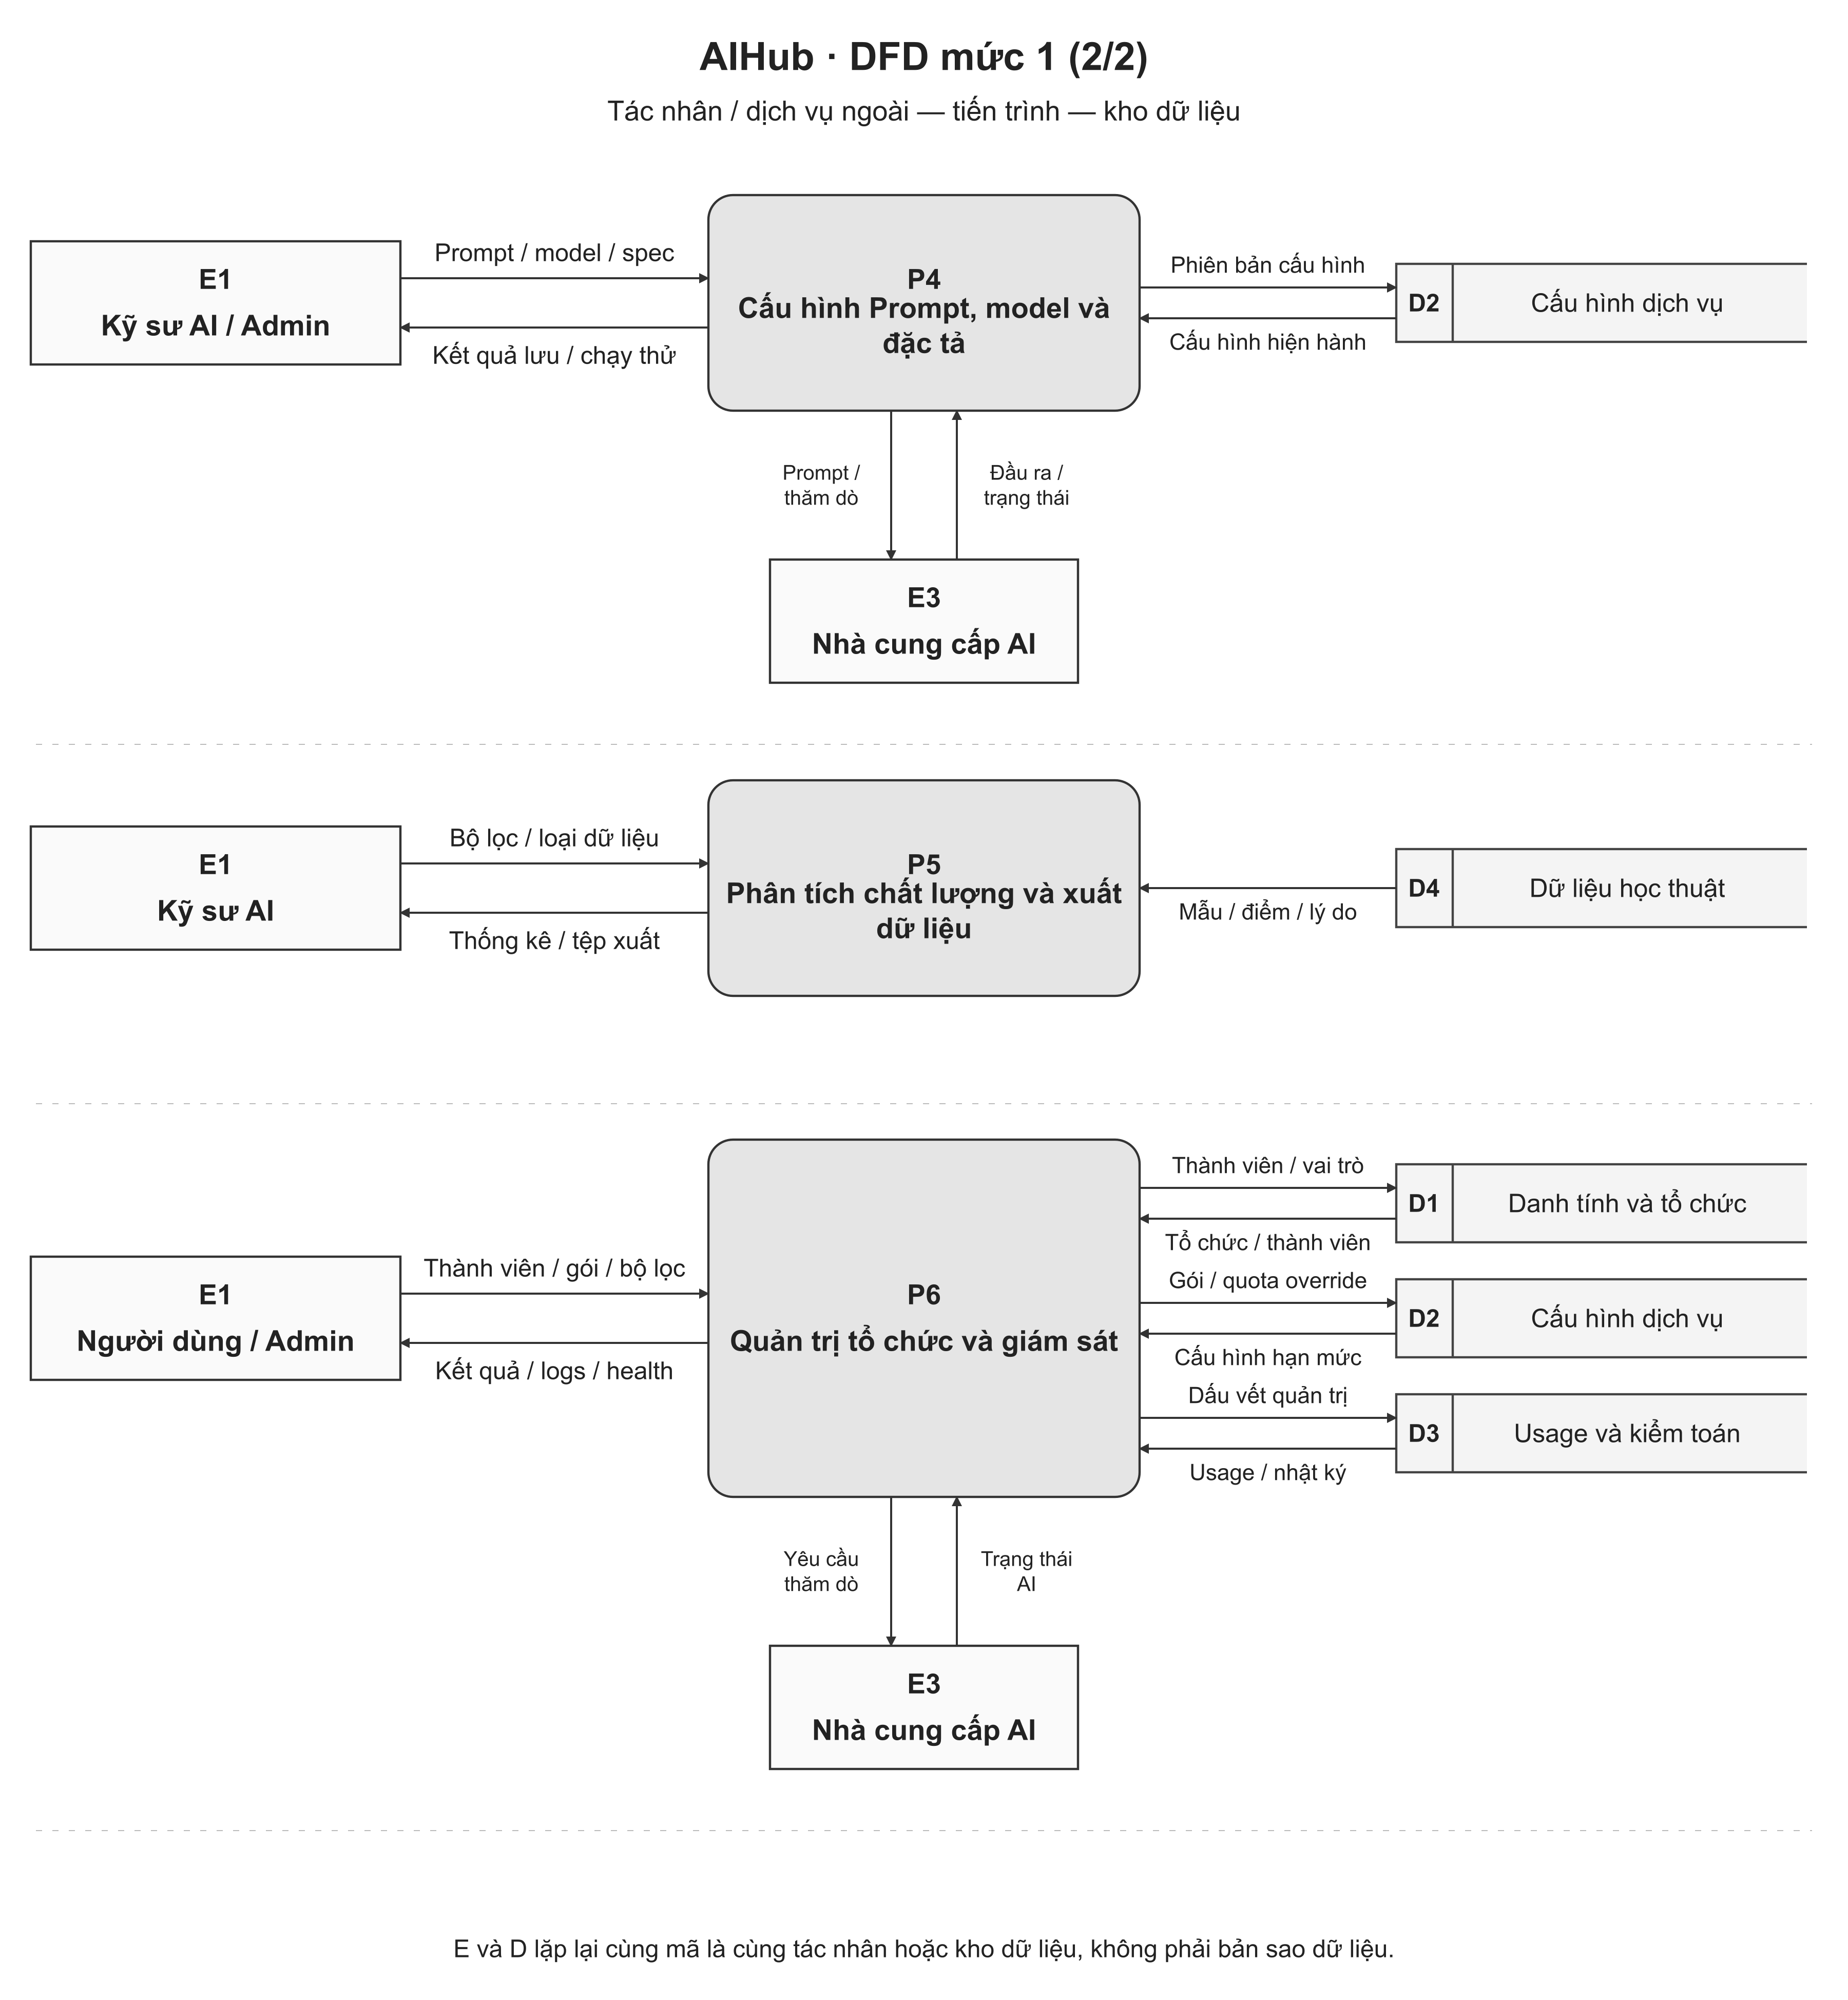
\includegraphics[width=\linewidth,height=0.78\textheight,keepaspectratio]{Images/DFD/AIHub/aihub_dfd_level1_2.png}
\caption{DFD mức 1 của AIHub: P4, P5, P6}
\label{aihub:fig:dfd-level1-2}
\end{figure}

\clearpage

\begin{longtable}{|p{0.22\linewidth}|p{0.72\linewidth}|}
\caption{Luồng dữ liệu mức 1 của AIHub}\label{aihub:tab:dfd-flows}\\
\hline
\textbf{Nguồn → Đích} & \textbf{Dữ liệu} \\
\hline
\endfirsthead
\hline
\textbf{Nguồn → Đích} & \textbf{Dữ liệu} \\
\hline
\endhead
E1 → P1 & Đăng nhập / thao tác khóa \\
\hline
P1 → E1 & Phiên / khóa mới \\
\hline
P1 → D1 & Phiên / mã băm khóa \\
\hline
D1 → P1 & Danh tính / vai trò \\
\hline
E2 → P2 & Credentials / payload \\
\hline
P2 → E2 & Bài tập / metadata \\
\hline
E1 → P2 & Sandbox / yêu cầu sinh \\
\hline
P2 → E1 & JSON / mẫu nháp \\
\hline
D1 → P2 & Khóa / quyền truy cập \\
\hline
D2 → P2 & Prompt / spec / quota \\
\hline
P2 → D3 & Usage / dấu vết \\
\hline
P2 → D4 & Mẫu AI nguyên bản \\
\hline
D4 → P2 & Dẫn chứng / ngữ cảnh \\
\hline
P2 → E3 & Prompt / tham số \\
\hline
E3 → P2 & Nội dung / metadata \\
\hline
E1 → P3 & Bộ lọc / bản hiệu đính \\
\hline
P3 → E1 & Dẫn chứng / trạng thái \\
\hline
P3 → D4 & Dẫn chứng / thẩm định \\
\hline
D4 → P3 & Mẫu / dẫn chứng cũ \\
\hline
P3 → E4 & Bộ lọc dẫn chứng \\
\hline
E4 → P3 & Dẫn chứng / lỗi \\
\hline
E1 → P4 & Prompt / model / spec \\
\hline
P4 → E1 & Kết quả lưu / chạy thử \\
\hline
P4 → D2 & Phiên bản cấu hình \\
\hline
D2 → P4 & Cấu hình hiện hành \\
\hline
P4 → E3 & Prompt / thăm dò \\
\hline
E3 → P4 & Đầu ra / trạng thái \\
\hline
E1 → P5 & Bộ lọc / loại dữ liệu \\
\hline
P5 → E1 & Thống kê / tệp xuất \\
\hline
D4 → P5 & Mẫu / điểm / lý do \\
\hline
E1 → P6 & Thành viên / gói / bộ lọc \\
\hline
P6 → E1 & Kết quả / logs / health \\
\hline
P6 → D1 & Thành viên / vai trò \\
\hline
D1 → P6 & Tổ chức / thành viên \\
\hline
P6 → D2 & Gói / quota override \\
\hline
D2 → P6 & Cấu hình hạn mức \\
\hline
P6 → D3 & Dấu vết quản trị \\
\hline
D3 → P6 & Usage / nhật ký \\
\hline
P6 → E3 & Yêu cầu thăm dò \\
\hline
E3 → P6 & Trạng thái AI \\
\hline
\end{longtable}


P3 lưu dẫn chứng vào D4 để P2 sử dụng khi sinh nội dung. Mẫu nguyên bản do P2 ghi vào D4 được P3 hiệu đính và thẩm định; P5 chỉ trích xuất dữ liệu phù hợp với loại tập huấn luyện được chọn. P2 và P6 cùng sử dụng D3 cho nhật ký và đối soát hạn mức. Sandbox của dịch vụ đối tác dùng dữ liệu mô phỏng trong P2, không phát sinh một lời gọi thật đến đối tác.

Deterministic Engine là thành phần dự phòng nội bộ của P2. Health check trong P6 kiểm tra kho dữ liệu nội bộ và nhận trạng thái từ nhà cung cấp AI; không xem PostgreSQL như một tác nhân ngoài.

Các luồng dữ liệu biên ở sơ đồ ngữ cảnh được phân bổ vào các tiến trình mức 1 tương ứng. Luồng đọc, ghi và phản hồi được thể hiện bằng các mũi tên riêng; sơ đồ không dùng điều kiện rẽ nhánh, nút bắt đầu hoặc kết thúc của activity diagram.
